%versi 3 (22-07-2020)
\chapter{Perancangan}
\label{chap:perancangan}
Bagian ini akan menjelaskan mengenai pernacangan yang digunakan untuk membangun perangkat lunak. 


\section{Perancangan Tabel Data Wilayah}
\label{sec:perancanganTabelDataWilayah}
Pada tabel data wilayah merupakan entitas utama dalam pengembangan perangkat lunak. Perancangan tabel data wilayah dapat dilihat dari tabel \ref{tab:tabelDataWilayah}.
\begin{table}[H]
	\centering
	\caption{Rancangan Tabel Data Willayah}
	\label{tab:tabelDataWilayah}
	\resizebox{\columnwidth}{!}{%
		\begin{tabular}{|l|l|c|c|c|c|c|c|}
			\hline
			\multicolumn{1}{|c|}{\textbf{No}} &
			\multicolumn{1}{c|}{\textbf{Atribut}} &
			\textbf{Tipe} &
			\textbf{Ukuran} &
			\textbf{Primary Key} &
			\textbf{Foreign Key} &
			\textbf{Null} &
			\textbf{Keterangan} \\ \hline
			1 & id                         & Integer & 11 & Yes & - & No & AUTO\_INCREMENT \\ \hline
			2 & nama\_kelurahan            & Varchar & 80 & -   & - & No & -               \\ \hline
			3 & luas\_kelurahan            & Float   & -  & -   & - & No & -               \\ \hline
			4 & luas\_kelurahan\_prediksi  & Float   & -  & -   & - & No & -               \\ \hline
			5 & luas\_rth\_kelurahan       & Float   & -  & -   & - & No & -               \\ \hline
			6 & persentase\_rth\_kelurahan & Float   & -  & -   & - & No & -               \\ \hline
			7 & link\_googlemapss          & Varchar & -  & -   & - & No & -               \\ \hline
		\end{tabular}%
	}
\end{table}


\section{Perancangan Kelas Controller}
\label{sec:perancanganController}
\begin{enumerate}
	\item \textit{function home}
	\begin{itemize}
		\item Masukan : -
		\item Keluaran: \textit{view} homePage
		\item Tabel yang diakses: data\_wilayah
		\item Deskripsi: Menampilkan halaman utama
		\item Algoritma: -
	\end{itemize}
\end{enumerate}
\section{Perancangan Antarmuka}
\label{sec:antarmuka}
Perancangan antarmuka pada perangkat lunak berguna untuk memudahkan pengguna memilih dan melihat hasil dari perbandingan kelurahan kota Bandung. Dalam gambar \ref{fig:rancanganAntarmuka}, terdapat desain antarmuka yang memungkinkan pengguna untuk memilih kelurahan di Kota Bandung. Pengguna dapat mengklik tautan \textit{Google Maps} sesuai dengan pilihan kelurahan, dan pengguna juga memiliki pilihan untuk melihat citra satelit kelurahan atau memilih citra satelit yang sudah di-segmentasi.

\begin{figure}[H]
	\centering
	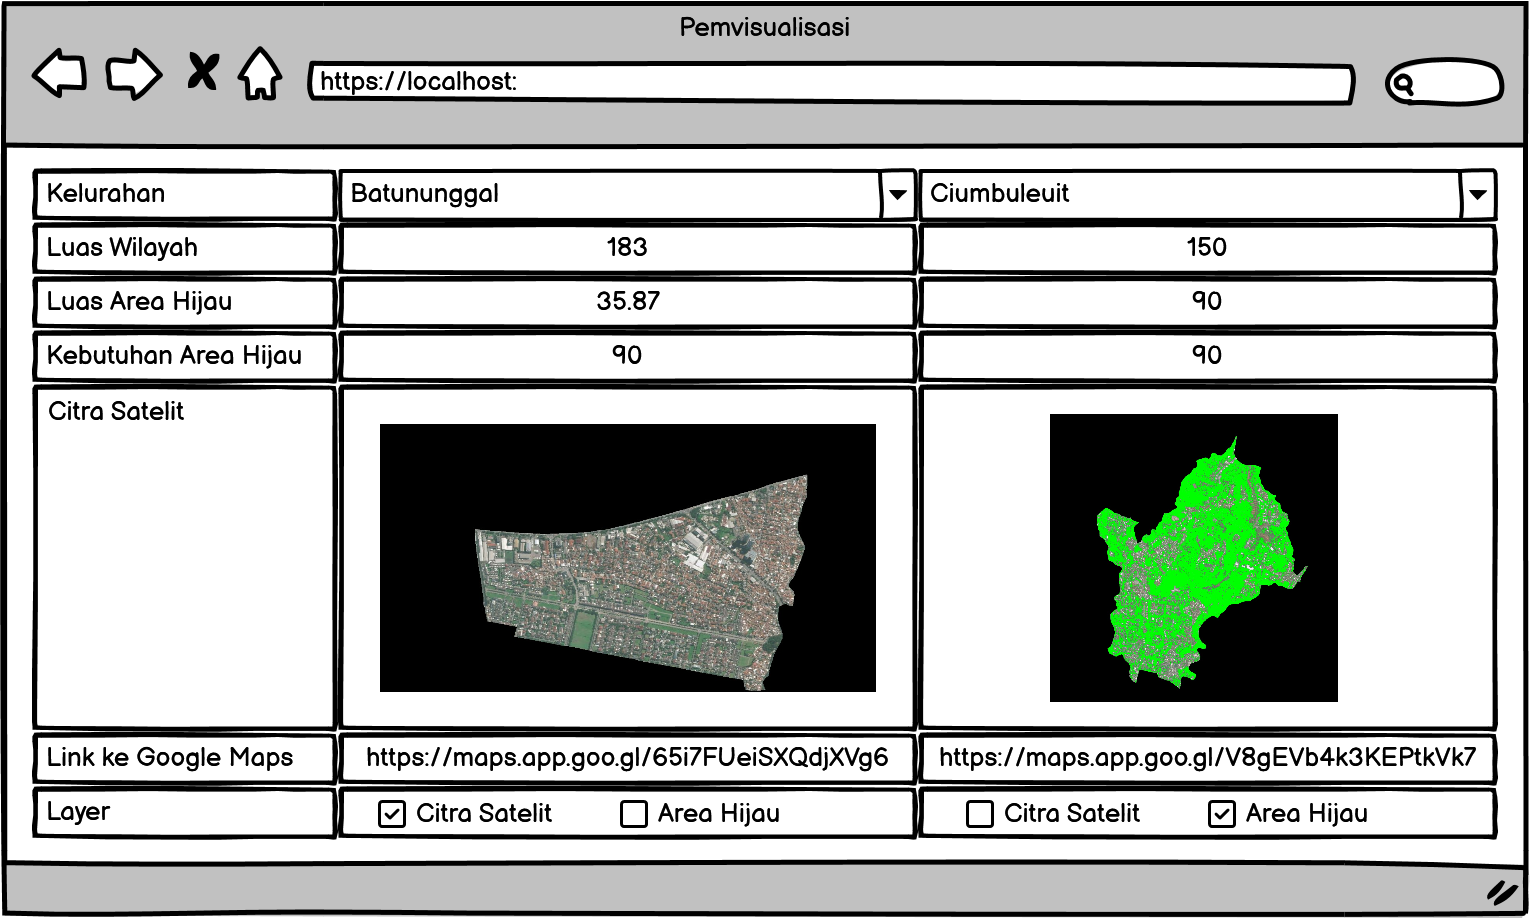
\includegraphics[width=0.8\textwidth]{Gambar/perancangan.png}
	\caption{Rancangan Antarmuka}
	\label{fig:rancanganAntarmuka}
\end{figure} 